Our previous study presented a parallel implementation of Dynamic Frontier (DF) Louvain \cite{sahu2024dflouvain}. In this work, we build upon that by applying the DF approach to parallel Leiden algorithm. We refer to this as \textbf{Dynamic Frontier (DF) Leiden}.

A straightforward application of the DF approach to the Leiden algorithm involves processing incrementally identified affected vertices during the local-moving phase of the algorithm, refining the obtained communities in the subsequent phase, aggregating the refined communities into a super-vertex graph (where each refined community is collapsed into a super-vertex), and repeating this process until convergence is reached. However, for small batch updates, convergence may occur after just one pass of the algorithm, at which point the algorithm would terminate. This results in suboptimal communities with low modularity, as the communities generated from the refinement phase did not have the opportunity to hierarchically merge and form tightly-knit groups with dense internal connections and sparse inter-community links. It is important to note that this issue does not arise in the absence of the refinement phase --- it occurs specifically when refinement is applied, as it forces the communities identified during the local-moving phase to be divided into smaller sub-communities. Despite this, we still aim to retain the refinement phase in the Leiden algorithm due to its beneficial properties, such as preventing the formation of poorly connected or even internally disconnected communities \cite{com-traag19}. To this end, unlike DF Louvain, we do not stop the algorithm after the first pass, but rather, run the algorithm until convergence occurs in a subsequent local-moving phase, where all vertices are processed, not just the affected ones. We refer to this method as \textbf{Full Refine}.

Nevertheless, for small batch updates, only a few communities may be impacted, and only those require refinement. To identify these communities, we track vertices that migrate between communities during the local-moving phase and mark both the source and target communities as changed, i.e., to be refined --- these communities may have altered sub-community structures. However, the community membership ID assigned to each vertex from the local-moving phase may not always be consistent; for example, community $c$ might not contain a vertex with ID $c$, as it could have migrated to another community. This inconsistency could cause issues during the refinement phase, where each vertex, in the communities to be refined, must initially belong to its own community. To understand this, consider an example. Say we break up the community, the vertex with ID $c$ belong to (for refinement), but do not break up the community $c$, vertex $c$ could continue to stay as an isolated community, while not being connected to any of the vertices in community $c$. Worse still, it is possible that two separate communities with the same ID $c$ are formed, while not being connected. It should be noted that this problem does not occur if we refine or break up all communities, but rather arises only if we refine a subset of communities. To resolve this, we must renumber communities such that the vertex with ID $c$ is part of community $c$, or in other words, by renumbering each community $c$ to an new community ID $i$, where $i$ is one of the constituent vertices of community $c$. In addition, we must accordingly adjust the total community edge weights and changed community flags, since these are populated based on the old community IDs.

Next, we consider the impact of batch updates on the communities requiring refinement. Edge deletions within a community can cause it to split. However, if a community is isolated, the local-moving phase cannot find better community assignments for any of the vertices belonging to the community. Therefore, refinement is the only way for such communities to split. Since community migrations do not occur, these communities would not be marked for refinement. To address this, for edge deletions in the batch update belonging to the same community, we mark the community as changed --- ensuring it is refined after the local-moving phase. Similarly, edge insertions affecting different parts of a community might also lead to a split, and must therefore be refined. Accordingly, for edge insertions in the batch update belonging to the same community, we mark the community as changed. We refer to this method of selective refinement of communities obtained from he local-moving phase of the algorithm, considering both vertex migration and the batch update, as \textbf{Subset Refine}. Note that selective refinement is performed only in the first pass of Leiden algorithm --- in the remaining passes, all the communities are refined.

However, the above selective refinement method hardly improves the performance of the DF Leiden, particularly for small batch updates. For these smaller updates, the aggregation phase remains a major bottleneck. This is mainly due to the selective refinement of communities, which results in a large difference in the sizes of communities to be aggregated --- the refined communities tend to be small, while the unrefined communities tend to be large. This creates a heavy workload for threads aggregating these unrefined communities into super-vertices. To ensure better load balancing, heavily loaded threads should be assigned minimal additional communities. Dynamic work scheduling can help, with each thread being assigned a smaller range of community IDs, or chunks. However, chunk sizes that are too small can introduce significant scheduling overhead. Through experimentation with chunk sizes from $1$ to $2048$ --- on large graphs (given in Table \ref{tab:dataset-large}), with uniformly random batch updates consisting of $80\%$ edge insertions and $20\%$ edge deletions (see Section \ref{sec:batch-generation}), on batch sizes of $10^{-7}|E|$, $10^{-5}|E|$, and $10^{-7}|E|$, where $|E|$ is the number of edges in the original graph --- we find that a chunk size of $32$ provides the best overall performance for ND, DS, and DF Leiden; as shown in Figure \ref{fig:aggregation-adjust-chunksize}. We refer to this method as \textbf{Optimized Aggregation}.

Figure \ref{fig:optimize-subrefine} illustrates the mean runtime of DF Leiden based on the three methods mentioned, \textit{Full Refine}, \textit{Subset Refine}, and \textit{Optimized Aggregation} --- on large graphs with\ignore{uniformly random} batch updates consisting of edge insertions and deletions, of size $10^{-7}|E|$ to $0.1|E|$.

The pseudocode for \textit{Optimized Aggregation} DF Leiden, which we from here on refer to simply as DF Leiden, is presented in Algorithm \ref{alg:frontier}, with a detailed explanation provided in Section \ref{sec:our-frontier}. In addition to DF Leiden, we also apply the \textit{Optimized Aggregation} method to ND and DS Leiden. The corresponding pseudocode for these algorithms is given in Algorithms \ref{alg:naive} and \ref{alg:delta}, with explanations found in Sections \ref{sec:our-naive} and \ref{sec:our-delta}, respectively. Similar to DF Louvain, we use the weighted degrees of vertices and the total edge weights of communities as auxiliary information, as illustrated in Figure \ref{fig:about-auxiliary}. For simplicity, we do not skip the aggregation phase of Leiden algorithm, even if a small number of communities are being merged together, unlike our original implementation of Static Leiden \cite{sahu2023gveleiden}. This allows us to maintain high quality\ignore{obtained} communities, with a small sacrifice in terms of runtime --- for Static, ND, DS, and DF Leiden.

\begin{figure}[!hbt]
  \centering
  \subfigure{
    \label{fig:optimize-subrefine--8020}
    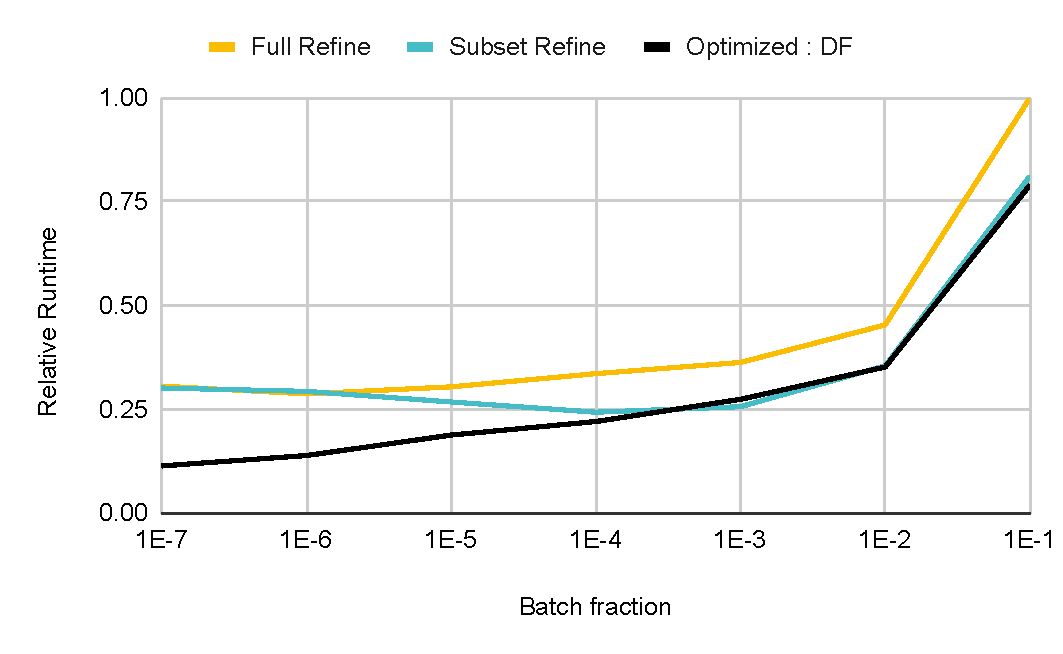
\includegraphics[width=0.98\linewidth]{out/optimize-subrefine-8020.pdf}
  } \\[-2ex]
  \caption{Mean Runtime and Modularity of communities obtained with our multicore implementation of \textit{Static}, \textit{Naive-dynamic (ND)}, \textit{Delta-screening (DS)}, and \textit{Dynamic Frontier (DF)} Leiden on real-world dynamic graphs, using batch updates of size $10^{-5}|E_T|$ to $10^{-3}|E_T|$. Here, (a) and (b) display the overall runtime and modularity across all temporal graphs, while (c) and (d) display the runtime and modularity for each individual graph. In (a), the speedup of each approach relative to Static Leiden is labeled.}
  \label{fig:optimize-subrefine}
\end{figure}

\begin{figure}[!hbt]
  \centering
  \subfigure[Relative runtimes on uniformly random batch updates of size $10^{-7}|E|$]{
    \label{fig:aggregation-adjust-chunksize--batch7}
    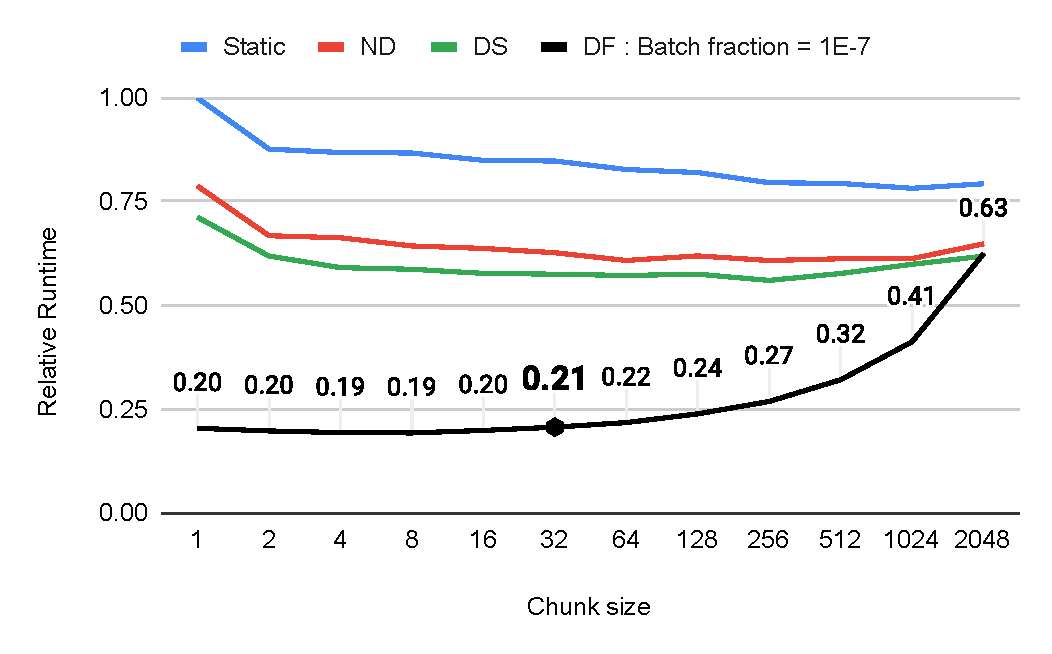
\includegraphics[width=0.98\linewidth]{out/aggregation-adjust-chunksize7.pdf}
  }
  \subfigure[Relative runtimes on uniformly random batch updates of size $10^{-5}|E|$]{
    \label{fig:aggregation-adjust-chunksize--batch5}
    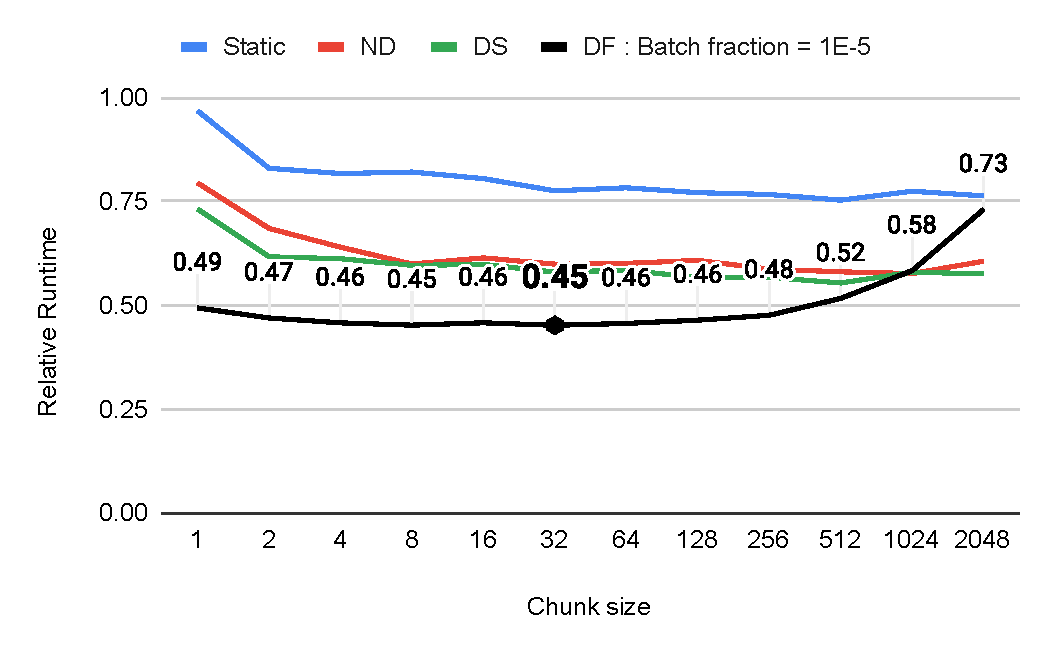
\includegraphics[width=0.98\linewidth]{out/aggregation-adjust-chunksize5.pdf}
  }
  \subfigure[Relative runtimes on uniformly random batch updates of size $10^{-3}|E|$]{
    \label{fig:aggregation-adjust-chunksize--batch3}
    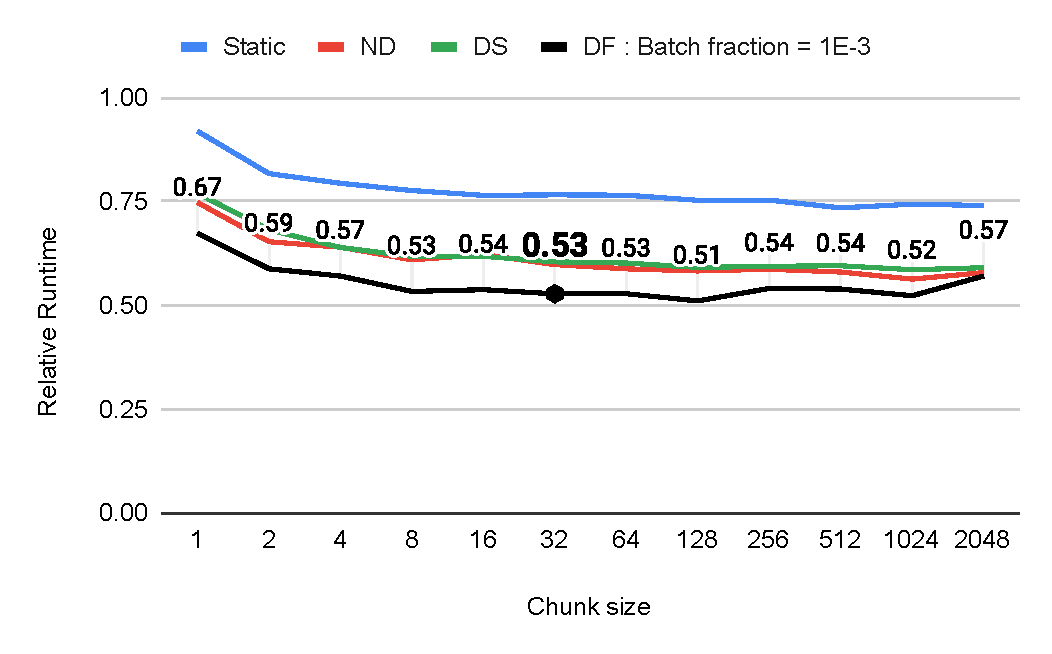
\includegraphics[width=0.98\linewidth]{out/aggregation-adjust-chunksize3.pdf}
  } \\[-1ex]
  \caption{Relative Runtime of \textit{Static}, \textit{Naive-dynamic (ND)}, \textit{Delta-screening (DS)}, and \textit{Dynamic Frontier (DF)} Leiden, with varying dynamic schedule chunk size (OpenMP), for aggregation phase of the Leiden algorithm. These tests were conducted on large graphs, with batch updates randomly generated at sizes of $10^{-7}|E|$, $10^{-5}|E|$, and $10^{-3}|E|$. The results suggest that a chunk size of $32$ is optimal (highlighted).}
  \label{fig:aggregation-adjust-chunksize}
\end{figure}

\begin{figure}[hbtp]
  \centering
  \subfigure{
    \label{fig:about-auxiliary--with}
    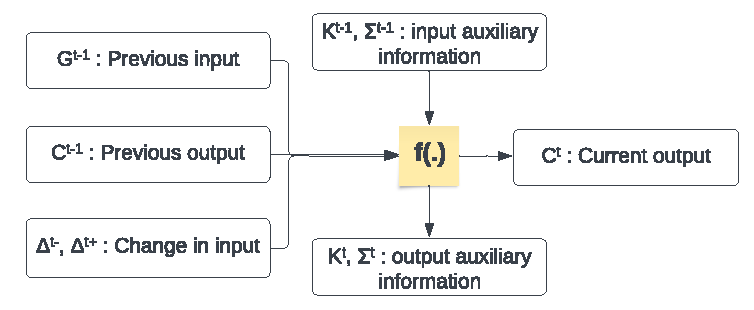
\includegraphics[width=0.98\linewidth]{out/about-auxiliary-with.pdf}
  } \\[-2ex]
  \caption{A dynamic community detection algorithm $f(.)$ takes as input the previous graph $G^{t-1}$, community memberships $C^{t-1}$, and the batch update $\Delta^{t-}$, $\Delta^{t+}$, and produces the updated community memberships $C^t$. However, it may also consider additional information such as the weighted degrees of vertices $K^{t-1}$ and the total edge weights of communities $\Sigma^{t-1}$ as auxiliary information, and yield updated auxiliary information $K^t$, $\Sigma^t$ \cite{sahu2024dflouvain}.}
  \label{fig:about-auxiliary}
\end{figure}

